%%%%%%%%%%%%%%%%%%%%%%%%%%%%%%%%%%%%%%%%%%%%%%%%%%%%%%%%%%%%%%%%%%%%%%%%%%%%%%%%
%
%   Semester project, fall term 2014
%   Author: Jakob Ehrl, born 01/24/91
%   Study program: Computer science, MA 1
%   
%   Professor Dr. Francesco Mondada
%   Assistant: Dr. Stefan Witwicki
%
%%%%%%%%%%%%%%%%%%%%%%%%%%%%%%%%%%%%%%%%%%%%%%%%%%%%%%%%%%%%%%%%%%%%%%%%%%%%%%%%%

\chapter{Introduction}

\section{Description of the challenge}
This competition involves 5 teams of 3 students coming from different sections and aims to challenge the students in building  an autonomous mobile robot for PET bottles collection and transport in a reserved area.
In the figure below (Figure 1) is represented the 8mx8m arena where the robot will have to work.
As it can be noticed, the arena is divided in 4 differents zones and, according to the difficulty to access or to perform in the zone, the weight in terms of points accorded for each bottle collected is different.

\begin{figure}[H]
  \centering
  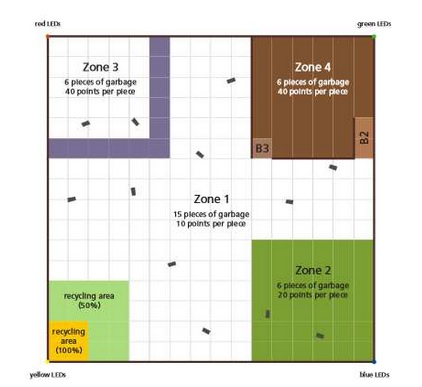
\includegraphics[width=0.6\textwidth]{Arena.jpg}
  \caption{Arena configuration.}
\label{fig:Arena}
\end{figure}

After being picked up the PET bottles need to be transported to a 1mx1m recycling area (left-down corner in Figure 1) in order to be awarded with the 100\% of the points given by the bottles.
If they were to be released within the second limit of the recycling area they would be worth 50\% of the points. Finally if they were to be kept within the robot the amounts in points would be 25\% of the actual value of the collected bottle. 

\section{Division of labor}
In order to speed up the robot’s process of realization we have distributed the principal tasks among the components of the team.
The  three main aspects that have been singularly developed, although always being in contact with the others team members in order to advance toward a harmonious final result, are:
\begin{itemize}
\item Mechanical Part
\item Electronic Part
\item Software Part
\end{itemize}

Deadlines on achievements for each single part were defined according to Gantt charts that helped us to keep an overall look on the advancement of the project.
In figure \ref{fig:GanttChart1} is represented the first Gantt chart conceived after the decision on the main characteristics of the robot and previous to the last milestone were all the details behind our idea of the robot were to be discussed with the supervisors.

\begin{figure}[H]
 \centering
 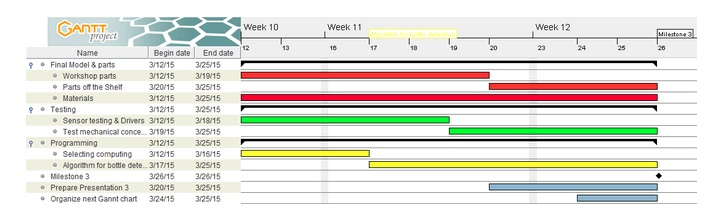
\includegraphics[width=1\textwidth]{GanttChart1.jpg}
 \caption{Work plan antecedent to the 3th milestone.}
\label{fig:GanttChart1}
\end{figure}


Another Gantt chart has been realized after the 3th milestone in order to organize the final work and it is showed in the figure \ref{fig:GanttChart2} below.

\begin{figure}[H]
 \centering
 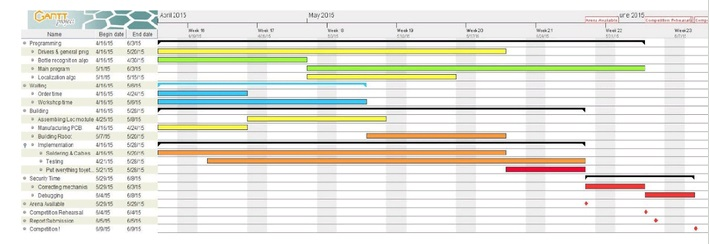
\includegraphics[width=1\textwidth]{GanttChart2.jpg}
 \caption{Gantt chart until the end.}
\label{fig:GanttChart2}
\end{figure}


As already said the division of the development of the robot in mechanical, electronic and software aspect was necessary to speed up the realization of the robot, although the lasts weeks have been dedicated to the merging of these differents parts allowing the team to work on the mechatronic of the robot and finally obtaining it with all the characteristics that had emerged during the initial brainstorming and developed during the advancement of the single parts.

\chapter{Research}

%\section{Ideas}
%some drawings and stuff from the main ideas in the %beginning

\section{Selection process}

%(The tables where we chose the features of the robot, and the cahier des charges that we should respect)

Firstly, as a group, we evaluated all the possible strategies that could lead to the achievement of the goal.
In the following, can be found in a schematic way the morphological charts of all the solutions that have been evaluated as well as the choices that brought us to the final design of our robot that will be treated in the following section.

This first morphological chart analyzes the possible solutions that we evaluated for the robot’s locomotion. In particular, the wheeled solutions, refer to the use of the Wild thumper chassis that can be modified exploiting either 4 or 6 wheels. This chassis was the one present in the catalogue, therefore the easiest to obtain. Furthermore this kind of structure had been used also in the previous editions of the competition and this was a good basis in terms of experience to begin with.
Others solutions like rubber tracks and swedish wheels have been evaluated.
However, as depicted in the related morphological chart, the advantages in using the Wild Thumper chassis with 4 wheels resulted more appealing to us, in particular its polyvalence, making us pick up this solution for the robot’s locomotion.

\begin{figure}[H]
 \centering
 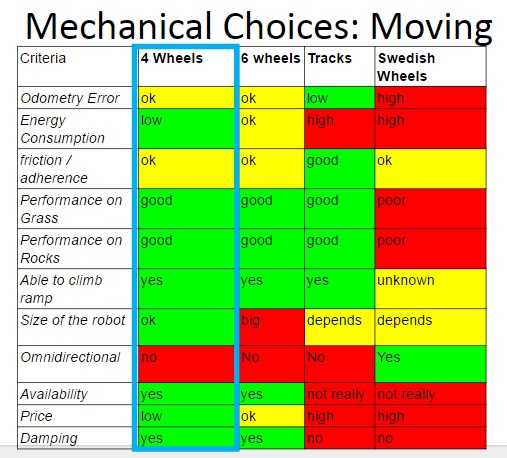
\includegraphics[width=0.7\textwidth]{MechanicalChoises.jpg}
 \caption{Morphological chart of the mechanical criteria.}
\label{fig:MechanicalChoises}
\end{figure}

Being the bottles’ collection the objective of the competition, right after choosing the locomotion method we started evaluating the possible solutions to accomplish this goal.
The first evaluation we made has been about the principle behind the system.
Indeed there are two possible approaches to the achievement of this task:

\begin{itemize}
\item Selective Approach
\item Greedy Approach
\end{itemize}

In a selective approach, each bottle has to be detected and, furthermore, its position and orientation need to be computed in order to approach the PET bottle in the desired way and grasping it by mean of a robotic arm or another precise pick up system.
However, this kind of solution, even if fascinating, appeared to us as a constraint and would have inevitably led to a waste of time. Obviously, this resulted to us as a not fitting solution for a competition that is limited to 10 minutes, thus we pointed toward a more greedy approach.
In a greedy approach, indeed, bottles don’t need to be perfectly identified and they could be picked up also by only being in the path of the robot.
With this idea in mind we started evaluating the mechanic systems that could provide such a favorable behavior.
The evaluated solutions are shown in the morphological chart in Figure t.
In our case we have chosen to couple a rigid elevator, which aims to pick up the bottle from the terrain putting it in a storage area upon the robot, with a rotating sponge, represented in figure r that aims to push the bottle within the elevator and avoid to make it exit once entered. 

\begin{figure}[H]
 \centering
 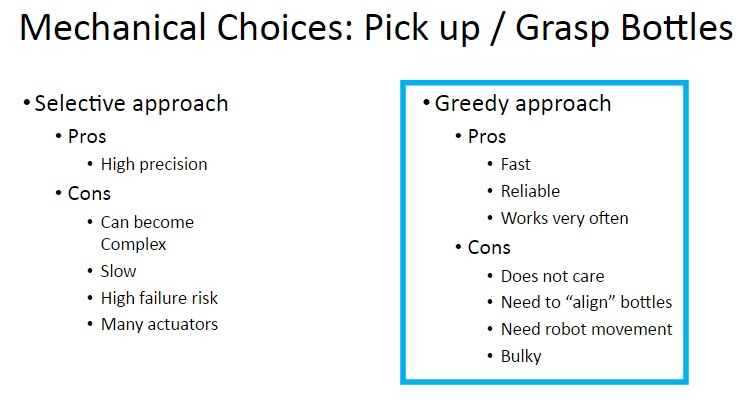
\includegraphics[width=0.9\textwidth]{PickUpApproach.jpg}
 \caption{Possible approaches for picking up a bottle.}
\label{fig:PickUpApproach}
\end{figure}

\begin{figure}[H]
 \centering
 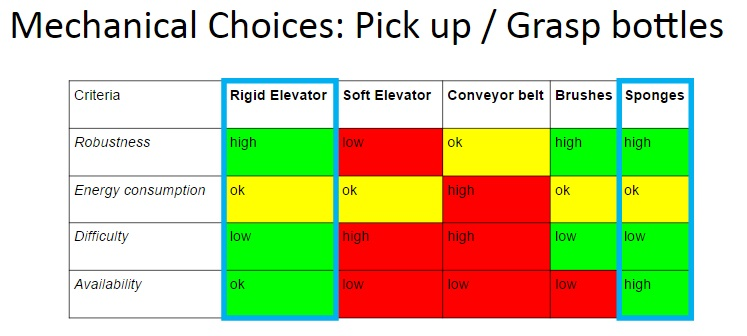
\includegraphics[width=0.9\textwidth]{PickUpChoises.jpg}
 \caption{Morphological chart of the picking up criteria.}
\label{fig:PickUpChoises}
\end{figure}

As already said the bottles, once collected, are placed in a storage area disposed on the robot chassis. Evaluating the criteria depicted in the morphological chart in figure s we opted for an unorganized storage of medium size.
\begin{figure}[H]
 \centering
 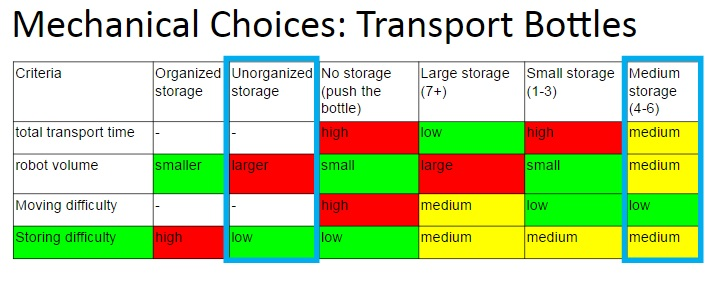
\includegraphics[width=0.8\textwidth]{TransportBottles.jpg}
 \caption{Morphological chart of the possible solutions to transport the bottles.}
\label{fig:TransportBottles}
\end{figure}

Finally, in figure e is shown the morphological chart that made us choose the sensors that allows the robot to perceive the environment and detect the bottles.                                                
\begin{figure}[H]
 \centering
 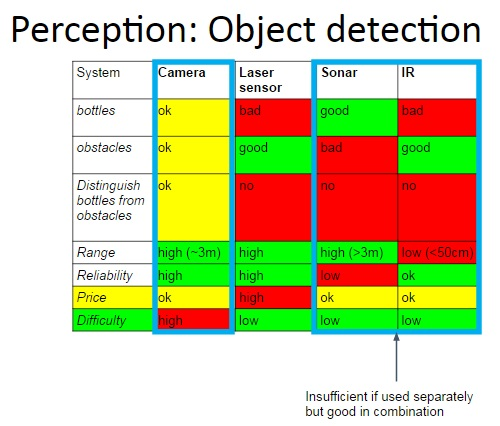
\includegraphics[width=0.7\textwidth]{ObjectDetection.jpg}
 \caption{Morphological chart for the sensors' choice.}
\label{fig:ObjectDetection}
\end{figure}

%\section{Choices} 
%Choices that we did, justifications and when we %changed our minds..